\documentclass[12pt]{article}
\usepackage{amsfonts}
\usepackage{fancyhdr}
\usepackage{comment}
\usepackage[a4paper, top=1cm, bottom=1.5cm, left=2cm, right=2cm]{geometry}
\usepackage{enumitem}
\usepackage{times}
\usepackage{changepage}
\usepackage{amssymb}
\usepackage{graphicx}
\usepackage{tabularx}
\usepackage{titlesec}
\usepackage{changepage}
\usepackage[parfill]{parskip}
\usepackage{wrapfig}
\usepackage[export]{adjustbox}
\usepackage{multirow}
\usepackage{array}
\usepackage[table]{xcolor}
\usepackage{longtable,booktabs}
\usepackage{float}
\usepackage{listings} % For presenting code nicely
\usepackage{hyperref}
\usepackage{framed}

\hypersetup{
    colorlinks,
    citecolor=black,
    filecolor=black,
    linkcolor=black,
    urlcolor=black
}

% settings %
\setcounter{secnumdepth}{3} % enumerate
\setcounter{tocdepth}{3}    % TOC entries
\renewcommand{\contentsname}{Innholdsfortegnelse}
\titlespacing*{\paragraph}{\parindent}{1ex}{1em}

% counters %
\newcounter{figurecounter}

% commands %
\newcommand*{\FigureCounter}{\stepcounter{figurecounter}\textit{Figur \arabic{figurecounter}}}
\newcommand{\txt}[1]{\FigureCounter\begin{shaded}\lstinputlisting[language={}]{#1}\end{shaded}}
\newcommand{\code}[2]{\FigureCounter\begin{shaded}\lstinputlisting[language=#1]{#2}\end{shaded}}

% colors %
\definecolor{pblue}{rgb}{0.13,0.13,1}
\definecolor{pgreen}{rgb}{0,0.5,0}
\definecolor{pred}{rgb}{0.9,0,0}
\definecolor{pgrey}{rgb}{0.46,0.45,0.48}
\definecolor{ccBorder}{HTML}{ccc9c0}
\definecolor{ccInner}{HTML}{edf3f5}
\definecolor{ccFrame}{HTML}{f2eee4}
\definecolor{shadecolor}{named}{ccFrame} 

% lstset %
\lstset{
    language=Java,
    showspaces=false,
    showtabs=false,
    aboveskip=3mm,
    belowskip=3mm,
    breaklines=true,
    showstringspaces=false,
    breakatwhitespace=true,
    columns=fullflexible,
    frame=single,
    commentstyle=\color{pgreen},
    keywordstyle=\color{pblue},
    stringstyle=\color{pred},
    basicstyle=\footnotesize\ttfamily,
    moredelim=[is][\textcolor{pgrey}]{\%}{\%}
    postbreak=\mbox{\textcolor{red}{$\hookrightarrow$}\space}
}
\begin{document}
\title{Big Data - Prosjekt}
\author{%
    Gruppe 0013:\\
    Mats Engelien, studentnr: 192288\\
    Lars Erik Faber, studentnr: 193173}
\date{}
\maketitle
\begin{center}
    
\includegraphics[scale=1]{images/world_education.jpg}    
\end{center}
\thispagestyle{empty}
\newpage
\tableofcontents
\thispagestyle{empty}
\newpage
\setcounter{page}{1}

\textbf{GitHub} repoet vårt er Public og finnes her: https://github.com/larseriktf/BigData

\section{Milepæl 2}
\subsection{Introduksjon}
I denne milepælen har vi funnet et nytt datasett til nettsiden vår. Vi har gått bort ifra musikk-konseptet fra tidligere milepæl, da det ikke var gunstig for funksjonalitet på nettsiden. Datasettet vi har valgt for KV-store inneholder data fra undersøkelser gjort på to skoler i Portugal for å se hvordan studentene opptrer på skolen. Datasettet heter Student Performance Data Set og kan finnes her:

Datasett: https://www.kaggle.com/larsen0966/student-performance-data-set/version/2

\subsection{Hvordan kommer data inn?}
Databasen vi har valgt tar utgangspunktet i et datasett som bruker data fra en undersøkelse på studenter fra to skoler i Portugal. For at ny data skal bli lagt inn i databasen, må det gjøres enda en undersøkelse ved enten de samme skolene eller en ny skole. Dataen må deretter legges inn via nettskjemaet med følgende felt på nettsiden

\begin{itemize}
  \item Skole
  \item Kjønn
  \item Alder
  \item Mors-utdanning
  \item Fars-utdanning
  \item Reisetid
  \item Studietid
  \item Stryk
  \item Skolestøtte
  \item Ekstratimer (Betalt)
  \item Aktiviteter utenom faget
  \item Internett
  \item Romantisk forhold
  \item Familie Relasjon
  \item Fritid
  \item Gå ut med venner
  \item Alkohol i ukedagene
  \item Alkohol i helgen
  \item Helse
  \item Fravær
  \item Karakter semester 1
  \item Karakter semester 2
  \item Sluttkarakter
\end{itemize}

Totalt er det 22 felt som må fylles ut, men når dette er sagt kommer mange av feltene til å ha standardverdier. I tillegg til nettskjemaet vil det være mulig å laste opp datasett i form av CSV eller JSON som har de samme kolonnene. Rader som er duplikater, vil ikke bli tatt hensyn til siden det er mulig å produsere de samme verdiene. Dette vil si at noen må manuelt legge til data via nettsiden for at dataen skal dukke opp i databasen, den vil ikke lytte etter endringer i datasettet via API-er.

\subsection{RIAK eller ETCD}
I prosjektet vårt har vi bestemt oss for å bruke ETCD, siden ETCD prioriterer konsistent data over tilgjengelighet. Dette er viktig, siden for dette prosjektet er det mye viktigere at dataen stemmer, enn å ha rask respons-tid. Hele hensikten med nettsiden er å forstå studiene som er tatt ved de forskjellige skolene, derfor må dataen være oppdatert. Siden CAP-teoremet gjelder i praksis kun når det oppstår en nodefeil, betyr det ikke at vi ofrer tilgjengelighet fullstendig, men det er mindre viktig i det tilfelle enn konsistens. Til slutt er det merkverdig å nevne at Riak er mye mer omfattende enn ETCD, derfor blir det også foretrukket i prosjektet.

\subsection{Design av nøkkel}
På grunn av måten vi velger å oppdatere eksisterende data i databasen, blir nøklene designet på en måte som skiller mellom komponenter og ny studentdata. Komponentene er JSON-objektene som brukes til å vise data på nettsiden, mens studentdataen er rådata som er nyttig for å holde dataen oppdatert. Hvis en student legges til eller oppdateres, oppdateres også komponentene i databasen. Den generelle strukturen på nøkkelen vil derfor være et prefiks for inndeling, etterfulgt av kolon, etterfulgt av navn eller id.

Verdier relatert til komponenter vil ha en nøkkel med prefiks "component" etterfulgt av navnet på komponenten. Eksempel på en nøkkel for en komponent i vår KV-store:

  component:studentByFreeTime

Verdier relatert til studenter vil ha nøkler med prefiks "student" etterfulgt av en 8-sifret id av typen Integer. Eksempel på en nøkkel for en student i vår KV-store:

  student:02381225

KV-store vil dermed følge en lignende struktur:

HER SKAL DET VÆRE EN TABELL FRA PDF-EN

\subsection{Design av dataobjekter og aggregeringer}
Som tidligere nevnt har vi delt opp dataobjektene i to grupper: komponenter og student-data. Grunnen til denne oppdelingen er for å optimalisere ytelse ved uthenting og oppdatering av data. Oppdelingen gjør det mulig å oppdatere individuelle komponenter ved å kun lese fra student-dataen som endret seg. Da unngår man å hente alle student-dataene for å oppdatere alle komponentene, og som resultat bruker nettsiden mindre kall til databasen.

\subsection{Ytelse og oppdatering av data}
På grunn av konsistens-kriterier for vår data, må read-kallene gjøres lineært som vil ta mer tid enn serialiserte kall. Ofte vil vi kun bruke et kall for å hente ut data, og heller bruke ytelsen til systemet for operasjoner på denne dataen.

En av grunnene til at dataen vil være lett tilgjengelig med få kall, er at den ikke nødvendigvis vil endre seg ofte (mange endringer heller i et kort tidsrom), men det er aggregeringene som gjøres med dataen som tar lang tid. Derfor er konsistens på dataen mye viktigere. Vi er avhengig av at dataen er korrekt og blir sjekket mot klyngen mer enn at uthenting av ny data er rask.

Ved første innlastning av nettsiden må den gjøre noen kall til databasen slik at den kan vise data på nettsiden. Siden det er 7 komponenter i denne nettsiden, har vi valgt å lagre hver komponent for seg i KV-store. Grunnen til dette er fordi hver komponent er ganske omfattende, og vi vil heller gjøre noen ekstra kall enn å laste et stort dataobjekt for hver oppdatering. Derfor blir det umiddelbart 7 kall mot KV-store når siden lastes inn.

Dersom vi ikke hadde designet dataen på denne måten, ville vi støtet på et problem dersom kun noen få studenter oppdateres. For eksempel med "averageGradesByStudyHours" komponentet i et datasett med 100 studenter, der 1 student endret verdi:

\begin{itemize}
  \item Hente alle studentobjekter fra databasen
  \item Bygge et averageGradesByStudyHours objektet på nytt
  \item Oppdater averageGradesByStudyHours i KV-store med den nye versjonen
  \item Oppdater studenten i KV-store med den nye versjonen
\end{itemize}

Det første steget ville bruke 100 kall, en for hver student, det tredje og fjerde steget er to kall. Til sammen blir dette 102 kall. Men siden vi har strukturert databasen ettersom, vil vi kunne minske dette tallet betraktelig. Med samme eksempel som over, her er måten vi gjør det på:

\newpage
\section{Milepæl 2}
\subsection{Introduksjon}
I denne milepælen har vi funnet et nytt datasett til nettsiden vår. Vi har gått bort ifra musikk-konseptet fra tidligere milepæl, da det ikke var gunstig for funksjonalitet på nettsiden. Datasettet vi har valgt for KV-store inneholder data fra undersøkelser gjort på to skoler i Portugal for å se hvordan studentene opptrer på skolen. Datasettet heter Student Performance Data Set og kan finnes her:

Datasett: https://www.kaggle.com/larsen0966/student-performance-data-set/version/2

\subsection{Hvordan kommer data inn?}
Databasen vi har valgt tar utgangspunktet i et datasett som bruker data fra en undersøkelse på studenter fra to skoler i Portugal. For at ny data skal bli lagt inn i databasen, må det gjøres enda en undersøkelse ved enten de samme skolene eller en ny skole. Dataen må deretter legges inn via nettskjemaet med følgende felt på nettsiden

\begin{itemize}
  \item Skole
  \item Kjønn
  \item Alder
  \item Mors-utdanning
  \item Fars-utdanning
  \item Reisetid
  \item Studietid
  \item Stryk
  \item Skolestøtte
  \item Ekstratimer (Betalt)
  \item Aktiviteter utenom faget
  \item Internett
  \item Romantisk forhold
  \item Familie Relasjon
  \item Fritid
  \item Gå ut med venner
  \item Alkohol i ukedagene
  \item Alkohol i helgen
  \item Helse
  \item Fravær
  \item Karakter semester 1
  \item Karakter semester 2
  \item Sluttkarakter
\end{itemize}

Totalt er det 22 felt som må fylles ut, men når dette er sagt kommer mange av feltene til å ha standardverdier. I tillegg til nettskjemaet vil det være mulig å laste opp datasett i form av CSV eller JSON som har de samme kolonnene. Rader som er duplikater, vil ikke bli tatt hensyn til siden det er mulig å produsere de samme verdiene. Dette vil si at noen må manuelt legge til data via nettsiden for at dataen skal dukke opp i databasen, den vil ikke lytte etter endringer i datasettet via API-er.

\subsection{RIAK eller ETCD}
I prosjektet vårt har vi bestemt oss for å bruke ETCD, siden ETCD prioriterer konsistent data over tilgjengelighet. Dette er viktig, siden for dette prosjektet er det mye viktigere at dataen stemmer, enn å ha rask respons-tid. Hele hensikten med nettsiden er å forstå studiene som er tatt ved de forskjellige skolene, derfor må dataen være oppdatert. Siden CAP-teoremet gjelder i praksis kun når det oppstår en nodefeil, betyr det ikke at vi ofrer tilgjengelighet fullstendig, men det er mindre viktig i det tilfelle enn konsistens. Til slutt er det merkverdig å nevne at Riak er mye mer omfattende enn ETCD, derfor blir det også foretrukket i prosjektet.

\subsection{Design av nøkkel}
På grunn av måten vi velger å oppdatere eksisterende data i databasen, blir nøklene designet på en måte som skiller mellom komponenter og ny studentdata. Komponentene er JSON-objektene som brukes til å vise data på nettsiden, mens studentdataen er rådata som er nyttig for å holde dataen oppdatert. Hvis en student legges til eller oppdateres, oppdateres også komponentene i databasen. Den generelle strukturen på nøkkelen vil derfor være et prefiks for inndeling, etterfulgt av kolon, etterfulgt av navn eller id.

Verdier relatert til komponenter vil ha en nøkkel med prefiks "component" etterfulgt av navnet på komponenten. Eksempel på en nøkkel for en komponent i vår KV-store:

  component:studentByFreeTime

Verdier relatert til studenter vil ha nøkler med prefiks "student" etterfulgt av en 8-sifret id av typen Integer. Eksempel på en nøkkel for en student i vår KV-store:

  student:02381225

KV-store vil dermed følge en lignende struktur:

HER SKAL DET VÆRE EN TABELL FRA PDF-EN

\subsection{Design av dataobjekter og aggregeringer}
Som tidligere nevnt har vi delt opp dataobjektene i to grupper: komponenter og student-data. Grunnen til denne oppdelingen er for å optimalisere ytelse ved uthenting og oppdatering av data. Oppdelingen gjør det mulig å oppdatere individuelle komponenter ved å kun lese fra student-dataen som endret seg. Da unngår man å hente alle student-dataene for å oppdatere alle komponentene, og som resultat bruker nettsiden mindre kall til databasen.

\subsection{Ytelse og oppdatering av data}
På grunn av konsistens-kriterier for vår data, må read-kallene gjøres lineært som vil ta mer tid enn serialiserte kall. Ofte vil vi kun bruke et kall for å hente ut data, og heller bruke ytelsen til systemet for operasjoner på denne dataen.

En av grunnene til at dataen vil være lett tilgjengelig med få kall, er at den ikke nødvendigvis vil endre seg ofte (mange endringer heller i et kort tidsrom), men det er aggregeringene som gjøres med dataen som tar lang tid. Derfor er konsistens på dataen mye viktigere. Vi er avhengig av at dataen er korrekt og blir sjekket mot klyngen mer enn at uthenting av ny data er rask.

Ved første innlastning av nettsiden må den gjøre noen kall til databasen slik at den kan vise data på nettsiden. Siden det er 7 komponenter i denne nettsiden, har vi valgt å lagre hver komponent for seg i KV-store. Grunnen til dette er fordi hver komponent er ganske omfattende, og vi vil heller gjøre noen ekstra kall enn å laste et stort dataobjekt for hver oppdatering. Derfor blir det umiddelbart 7 kall mot KV-store når siden lastes inn.

Dersom vi ikke hadde designet dataen på denne måten, ville vi støtet på et problem dersom kun noen få studenter oppdateres. For eksempel med "averageGradesByStudyHours" komponentet i et datasett med 100 studenter, der 1 student endret verdi:

\begin{itemize}
  \item Hente alle studentobjekter fra databasen
  \item Bygge et averageGradesByStudyHours objektet på nytt
  \item Oppdater averageGradesByStudyHours i KV-store med den nye versjonen
  \item Oppdater studenten i KV-store med den nye versjonen
\end{itemize}

Det første steget ville bruke 100 kall, en for hver student, det tredje og fjerde steget er to kall. Til sammen blir dette 102 kall. Men siden vi har strukturert databasen ettersom, vil vi kunne minske dette tallet betraktelig. Med samme eksempel som over, her er måten vi gjør det på:

\newpage
\section{Milepæl 3}

\subsection{Implementasjon av KV-database}
I denne milepælen har vi implementert noen komponenter fra forrige milepæl via Scala og SBT.

\subsubsection{Average Grades By Study Hours}
\textbf{PostAvgGradesByStudyHoursFromCSV.scala:}\\
\code{Scala}{code/milepael3/PostAvgGradesByStudyHoursFromCSV.scala}

\textbf{GetAvgGradesByStudyHours.scala:}\\
\code{Scala}{code/milepael3/GetAvgGradesByStudyHours.scala}

\FigureCounter
\begin{figure}[H]
  \centering
  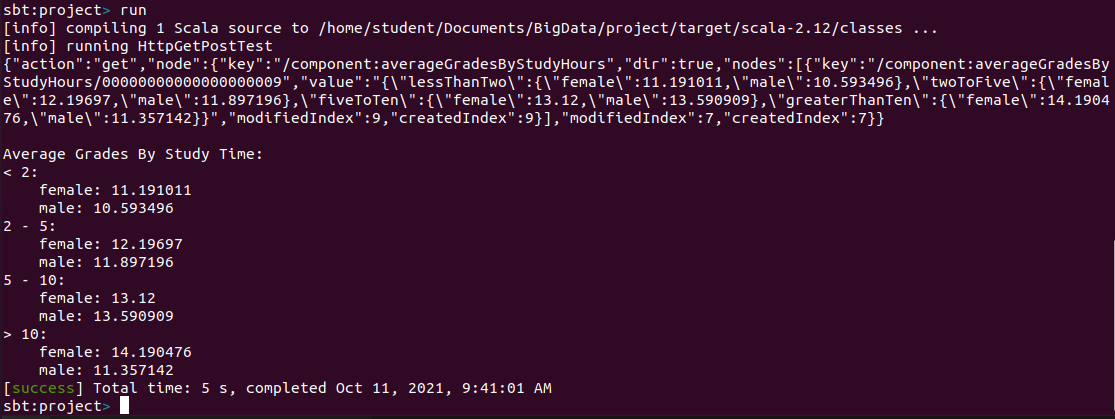
\includegraphics[width=\textwidth]{images/milepael3/GetAvgGradesByStudyHoursTerminal.png}
\end{figure}

\subsubsection{Students By Free Time}
\textbf{PostStudentsByFreeTimeFromCSV.scala}\\
\code{Scala}{code/milepael3/PostStudentsByFreeTimeFromCSV.scala}

\subsubsection{Average Grades By Parent Education}
\textbf{PostAvgGradesByStudentEduFromCSV.scala}\\
\code{Scala}{code/milepael3/PostAvgGradesByStudentEduFromCSV.scala}

\textbf{GetAvgGradesByParentEdu.scala}\\
\code{Scala}{code/milepael3/GetAvgGradesByParentEdu.scala}

\FigureCounter
\begin{figure}[H]
  \centering
  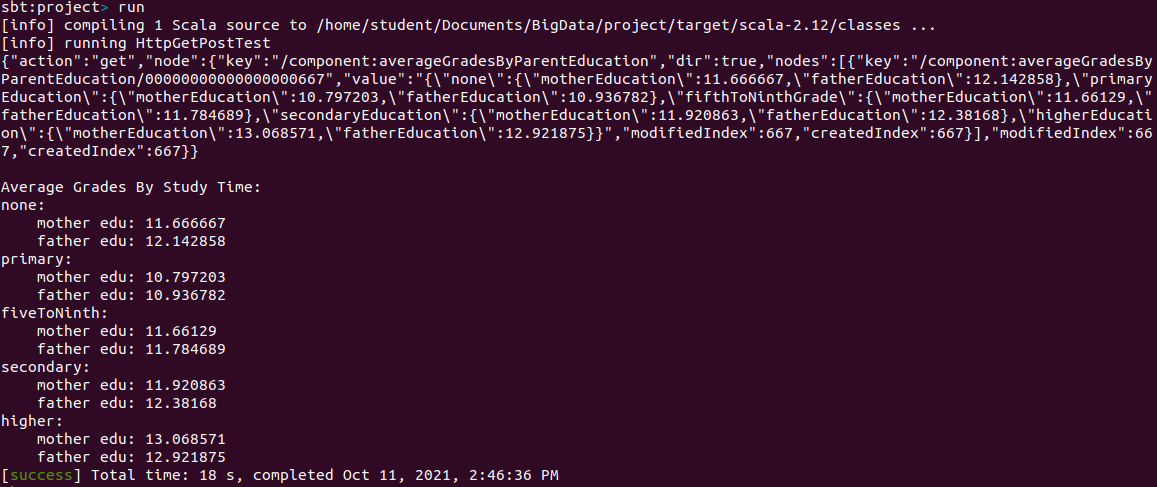
\includegraphics[width=\textwidth]{images/milepael3/GetAvgGradesByParentEduTerminal.png}
\end{figure}

\subsubsection{Student}
\textbf{PostStudentFromCSV.scala}\\
\code{Scala}{code/milepael3/PostStudentFromCSV.scala}

\textbf{AddStudent.scala}\\
\code{Scala}{code/milepael3/AddStudent.scala}
\subsection{Design Av Dokumentdatabase}
Her brukte vi datasettet "Socio-Economic Country Pofiles" fra Kaggle:

https://www.kaggle.com/nishanthsalian/socioeconomic-country-profiles

\subsubsection{Hvorfor kolonnedatabase?}
I hovedårsak er det gunstig å bruke dokument-orientert database med dette settet da vi kun trenger å organisere basert på land, og vil gjøre svært få kall mot databasen. Aggregeringene våre kan i flere tilfeller da ligge som referanser i hvert land, og vil heller eksistere som sine egne dokumenter. Ved endringer i datasettet vil aggregeringer kjøres på nytt, og endre verdiene i disse dokumentene. Grunnen til at dette kan være til fordel er hvor tungt det fort blir med mange kall mot dokument-orienterte databaser, så det viktigste blir konsistens på dataen. Når data oppdateres i her vil kun dokumentene som er påvirket av endringene ha operasjoner utført på de.

Mange aggregeringer er også mye raskere å få gjort i denne typen database da man henter ut et helt dokument ved spørringen, og alt informasjonen den inneholder. Dette gjør at man slipper å gjøre søk på tvers av tabeller eller må gjøre mere komplekse nøstede spørringer. I tillegg er det en veldig god modell for databaser som ikke gjør veldig mange endringer ofte, hvor tilgang til replika versjoner av data gir redundans ved mange spørringer og holder ytelsen oppe.

En av de aller mest interessante delene av denne typen database er indeksering, og hvordan det kan brukes for å gjøre at spørringer blir mye billigere. Indeksering tillater også da å lagre spørringer rett i RAM, men det krever at man har plass til hele settet man arbeider med også. I vår aggregering som tar inn brukerspesifiserte land og sammenligner kostnad kan potensielt være større da den kun trenger å holde det nyeste resultatet fra hver spørring.

\subsubsection{Country-Dokument}
\begin{itemize}
  \item Country: “CountryName”
  \item Population In Thousands: float
  \item GDP: float
  \item GDP Per capita: percent
  \item Unemployment: percent
  \item Labour Force Participation By Gender: percent
  \item PopGrowthRate Annual: Percentage
  \item Urban population: percent
  \item Urban population growth: avg annual precent%
  \item Health Total Expenditure: percent of GDP
  \item Education Total Expenditure: percent of GDP
  \item Education enrollment primary/secondary/tertiary: F/M per 100 pop
  \item Individuals using the internet: per 100 inhabitants
  \item CO2 emission estimates: million tons/tons per capita
  \item Pop. Using improved drinking water: Urban/rural %
  \item Quality of Life Index: float
  \item Purchasing power index: float
  \item Safety Index: float
  \item Health Care Index: int
  \item Cost of Living: float
  \item Cost of living index: float
  \item Property price to income Ratio: float
  \item Affordability index: float
  \item Cost of living plus rent index: float
  \item Life expectancy total: float
  \item Military expenditure: float
  \item Tax revenue: percent of GDP
\end{itemize}

\subsection{Aggregeringer}
% Aggregering 1 %
\subsubsection{Hva er verdens høyeste beskattende land etter GDP.}
Denne aggregeringen kan bli lagret i databasen som et eget dokument da det ikke er noe som endrer seg ofte. Dette gjør det lett å hente ut tabellen, og heller flere redundanskopier av dokumentet gjør at det blir lett tilgjengelig selv ved høy trafikk i databasen.

\FigureCounter
\begin{figure}[H]
  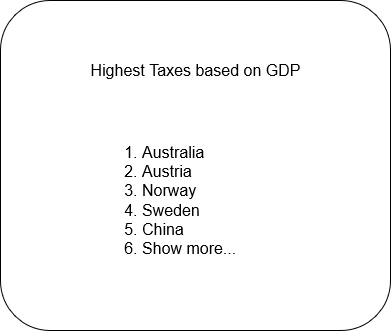
\includegraphics[scale=1]{images/milepael3/highestTaxesByGDP.png}
\end{figure}

\textbf{Pseudo-Kode}
\begin{enumerate}
  \item Hent ut alle land med skatt og GDP
  \item Sorter etter stor del av GDP som blir beskattet
  \item Post (legg inn referanse til aggregering i Land dokumenter)
\end{enumerate}

% Aggregering 2 %
\subsubsection{Livskvalitet etter skatt}
Denne aggregeringen er en av de mer komplekse vi har, denne spørringen gjøres mot en Multikey Index i landsdokumentene som gjør at den kun trenger å gjøre denne spørringen når data endrer seg. Alternativt kan spørringen lagres som et eget dokument med referanse til landene. Å lagre til dokument kan potensielt være billigere da man heller kan hente ut dette ved hver read, men å indeksere vil gjøre at færre interaksjoner vil skje med unødvendige dokumenter.

\FigureCounter
\begin{figure}[H]
  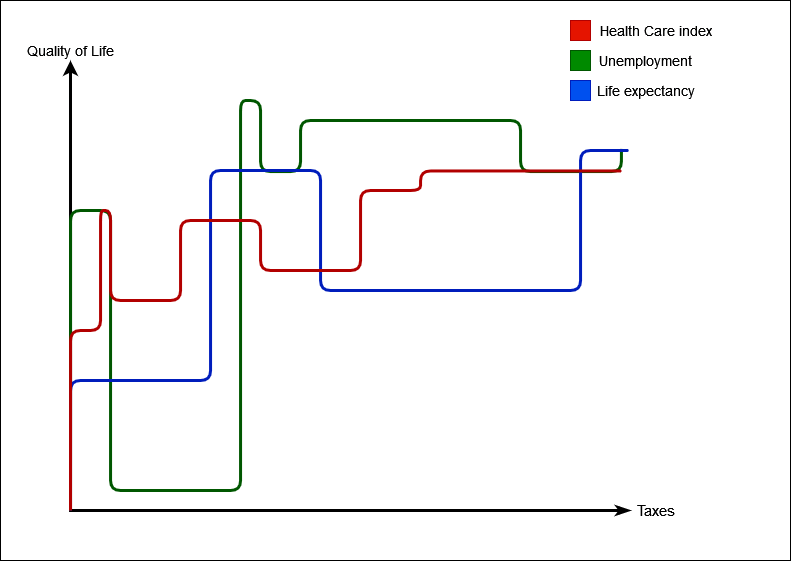
\includegraphics[scale=0.5]{images/milepael3/qualityOfLifeByTaxes.png}
\end{figure}

\textbf{Pseudo-Kode}
\begin{enumerate}
  \item Lag indeks
  \item Hent alle land sine quality of life verdier
  \item Lag objekter med disse verdiene
  \item Legg de sortert i en liste etter skatt i landet
  \item Post til dokument og legg referanse til referanse
\end{enumerate}

% Aggregering 3 %
\subsubsection{Land sammenlignet etter kost}
Denne aggregeringen er veldig billig ytelsesmessig med kun databasekall for å hente ut landene som blir valgt i menyene. Vi kan da kun sette nødvendige dokumenter i aggregeringspipelinen. Disse landene (…Y) kan da sjekkes mot verdien satt i hovedland(X), og så postes med riktig streng verdi. Dette kan gjøres via On-Demand Materialized Views.

Her vil det bli kjørt da n+1 spørringer mot databasen hvor n = antall Y. Det vil så bli aggregert fra pipeline som en array.

For denne spørringen gir det mening å bruke en indeks som har referanse til alle landsdokumentene. Å bruke indekser gjør at vi heller ser kun på dokumentene vi ønsker, i stedet for at alle dokumentene i samlingen må sjekkes.

\FigureCounter
\begin{figure}[H]
  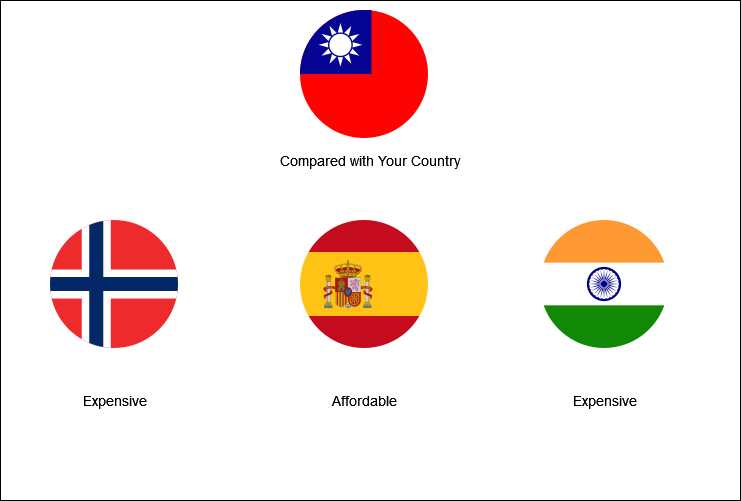
\includegraphics[scale=0.5]{images/milepael3/countriesComparedByExpensiveness.png}
\end{figure}

\textbf{Pseudo-Kode}
\begin{enumerate}
  \item Hent alle land og legg de i en liste
  \item Hent valgte lands navn og affordability index
  \item Hvis X sitt land er innen samme verdisone som Y = affordable
  \item Under = cheap
  \item Mer = expensive
  \item Post aggregering
\end{enumerate}

\subsection{Endring i data}
\begin{enumerate}
  \item Ny data kommer inn
  \item Landsdokumentene som blir påvirket vil endre informasjon
  \begin{itemize}
    \item Dokument-orienterte databaser vil kun gjøre endringer i dokumenter som blir påvirket av ny data, dersom det har skjedd endringer mot data som har vært indeksert vil det som regel være nødvendig å gjenskape indeksen
  \end{itemize}
  \item Aggregeringer og indekser som påvirkes og er lagret som dokument kjøres og lages på nytt
  \begin{itemize}
    \item Dette blir noe av det dyrere som skjer da aggregeringene kan gjøre mange databasekall, men dette vil være avhengig av hvor mange dokument som skal endres,
    og om endringene som er gjort påvirker de faktiske aggregeringene.
  \end{itemize}
  \item Id feltet vil måtte være det første feltet i en dokument, og rekkefølgen på feltene i objektet vil alltid være det samme så lenge en av endringene som skjer ikke omdøping av felt-navnene 
\end{enumerate}


\newpage
\section{Milepæl 2}
\subsection{Introduksjon}
I denne milepælen har vi funnet et nytt datasett til nettsiden vår. Vi har gått bort ifra musikk-konseptet fra tidligere milepæl, da det ikke var gunstig for funksjonalitet på nettsiden. Datasettet vi har valgt for KV-store inneholder data fra undersøkelser gjort på to skoler i Portugal for å se hvordan studentene opptrer på skolen. Datasettet heter Student Performance Data Set og kan finnes her:

Datasett: https://www.kaggle.com/larsen0966/student-performance-data-set/version/2

\subsection{Hvordan kommer data inn?}
Databasen vi har valgt tar utgangspunktet i et datasett som bruker data fra en undersøkelse på studenter fra to skoler i Portugal. For at ny data skal bli lagt inn i databasen, må det gjøres enda en undersøkelse ved enten de samme skolene eller en ny skole. Dataen må deretter legges inn via nettskjemaet med følgende felt på nettsiden

\begin{itemize}
  \item Skole
  \item Kjønn
  \item Alder
  \item Mors-utdanning
  \item Fars-utdanning
  \item Reisetid
  \item Studietid
  \item Stryk
  \item Skolestøtte
  \item Ekstratimer (Betalt)
  \item Aktiviteter utenom faget
  \item Internett
  \item Romantisk forhold
  \item Familie Relasjon
  \item Fritid
  \item Gå ut med venner
  \item Alkohol i ukedagene
  \item Alkohol i helgen
  \item Helse
  \item Fravær
  \item Karakter semester 1
  \item Karakter semester 2
  \item Sluttkarakter
\end{itemize}

Totalt er det 22 felt som må fylles ut, men når dette er sagt kommer mange av feltene til å ha standardverdier. I tillegg til nettskjemaet vil det være mulig å laste opp datasett i form av CSV eller JSON som har de samme kolonnene. Rader som er duplikater, vil ikke bli tatt hensyn til siden det er mulig å produsere de samme verdiene. Dette vil si at noen må manuelt legge til data via nettsiden for at dataen skal dukke opp i databasen, den vil ikke lytte etter endringer i datasettet via API-er.

\subsection{RIAK eller ETCD}
I prosjektet vårt har vi bestemt oss for å bruke ETCD, siden ETCD prioriterer konsistent data over tilgjengelighet. Dette er viktig, siden for dette prosjektet er det mye viktigere at dataen stemmer, enn å ha rask respons-tid. Hele hensikten med nettsiden er å forstå studiene som er tatt ved de forskjellige skolene, derfor må dataen være oppdatert. Siden CAP-teoremet gjelder i praksis kun når det oppstår en nodefeil, betyr det ikke at vi ofrer tilgjengelighet fullstendig, men det er mindre viktig i det tilfelle enn konsistens. Til slutt er det merkverdig å nevne at Riak er mye mer omfattende enn ETCD, derfor blir det også foretrukket i prosjektet.

\subsection{Design av nøkkel}
På grunn av måten vi velger å oppdatere eksisterende data i databasen, blir nøklene designet på en måte som skiller mellom komponenter og ny studentdata. Komponentene er JSON-objektene som brukes til å vise data på nettsiden, mens studentdataen er rådata som er nyttig for å holde dataen oppdatert. Hvis en student legges til eller oppdateres, oppdateres også komponentene i databasen. Den generelle strukturen på nøkkelen vil derfor være et prefiks for inndeling, etterfulgt av kolon, etterfulgt av navn eller id.

Verdier relatert til komponenter vil ha en nøkkel med prefiks "component" etterfulgt av navnet på komponenten. Eksempel på en nøkkel for en komponent i vår KV-store:

  component:studentByFreeTime

Verdier relatert til studenter vil ha nøkler med prefiks "student" etterfulgt av en 8-sifret id av typen Integer. Eksempel på en nøkkel for en student i vår KV-store:

  student:02381225

KV-store vil dermed følge en lignende struktur:

HER SKAL DET VÆRE EN TABELL FRA PDF-EN

\subsection{Design av dataobjekter og aggregeringer}
Som tidligere nevnt har vi delt opp dataobjektene i to grupper: komponenter og student-data. Grunnen til denne oppdelingen er for å optimalisere ytelse ved uthenting og oppdatering av data. Oppdelingen gjør det mulig å oppdatere individuelle komponenter ved å kun lese fra student-dataen som endret seg. Da unngår man å hente alle student-dataene for å oppdatere alle komponentene, og som resultat bruker nettsiden mindre kall til databasen.

\subsection{Ytelse og oppdatering av data}
På grunn av konsistens-kriterier for vår data, må read-kallene gjøres lineært som vil ta mer tid enn serialiserte kall. Ofte vil vi kun bruke et kall for å hente ut data, og heller bruke ytelsen til systemet for operasjoner på denne dataen.

En av grunnene til at dataen vil være lett tilgjengelig med få kall, er at den ikke nødvendigvis vil endre seg ofte (mange endringer heller i et kort tidsrom), men det er aggregeringene som gjøres med dataen som tar lang tid. Derfor er konsistens på dataen mye viktigere. Vi er avhengig av at dataen er korrekt og blir sjekket mot klyngen mer enn at uthenting av ny data er rask.

Ved første innlastning av nettsiden må den gjøre noen kall til databasen slik at den kan vise data på nettsiden. Siden det er 7 komponenter i denne nettsiden, har vi valgt å lagre hver komponent for seg i KV-store. Grunnen til dette er fordi hver komponent er ganske omfattende, og vi vil heller gjøre noen ekstra kall enn å laste et stort dataobjekt for hver oppdatering. Derfor blir det umiddelbart 7 kall mot KV-store når siden lastes inn.

Dersom vi ikke hadde designet dataen på denne måten, ville vi støtet på et problem dersom kun noen få studenter oppdateres. For eksempel med "averageGradesByStudyHours" komponentet i et datasett med 100 studenter, der 1 student endret verdi:

\begin{itemize}
  \item Hente alle studentobjekter fra databasen
  \item Bygge et averageGradesByStudyHours objektet på nytt
  \item Oppdater averageGradesByStudyHours i KV-store med den nye versjonen
  \item Oppdater studenten i KV-store med den nye versjonen
\end{itemize}

Det første steget ville bruke 100 kall, en for hver student, det tredje og fjerde steget er to kall. Til sammen blir dette 102 kall. Men siden vi har strukturert databasen ettersom, vil vi kunne minske dette tallet betraktelig. Med samme eksempel som over, her er måten vi gjør det på:

\newpage
\section{Milepæl 2}
\subsection{Introduksjon}
I denne milepælen har vi funnet et nytt datasett til nettsiden vår. Vi har gått bort ifra musikk-konseptet fra tidligere milepæl, da det ikke var gunstig for funksjonalitet på nettsiden. Datasettet vi har valgt for KV-store inneholder data fra undersøkelser gjort på to skoler i Portugal for å se hvordan studentene opptrer på skolen. Datasettet heter Student Performance Data Set og kan finnes her:

Datasett: https://www.kaggle.com/larsen0966/student-performance-data-set/version/2

\subsection{Hvordan kommer data inn?}
Databasen vi har valgt tar utgangspunktet i et datasett som bruker data fra en undersøkelse på studenter fra to skoler i Portugal. For at ny data skal bli lagt inn i databasen, må det gjøres enda en undersøkelse ved enten de samme skolene eller en ny skole. Dataen må deretter legges inn via nettskjemaet med følgende felt på nettsiden

\begin{itemize}
  \item Skole
  \item Kjønn
  \item Alder
  \item Mors-utdanning
  \item Fars-utdanning
  \item Reisetid
  \item Studietid
  \item Stryk
  \item Skolestøtte
  \item Ekstratimer (Betalt)
  \item Aktiviteter utenom faget
  \item Internett
  \item Romantisk forhold
  \item Familie Relasjon
  \item Fritid
  \item Gå ut med venner
  \item Alkohol i ukedagene
  \item Alkohol i helgen
  \item Helse
  \item Fravær
  \item Karakter semester 1
  \item Karakter semester 2
  \item Sluttkarakter
\end{itemize}

Totalt er det 22 felt som må fylles ut, men når dette er sagt kommer mange av feltene til å ha standardverdier. I tillegg til nettskjemaet vil det være mulig å laste opp datasett i form av CSV eller JSON som har de samme kolonnene. Rader som er duplikater, vil ikke bli tatt hensyn til siden det er mulig å produsere de samme verdiene. Dette vil si at noen må manuelt legge til data via nettsiden for at dataen skal dukke opp i databasen, den vil ikke lytte etter endringer i datasettet via API-er.

\subsection{RIAK eller ETCD}
I prosjektet vårt har vi bestemt oss for å bruke ETCD, siden ETCD prioriterer konsistent data over tilgjengelighet. Dette er viktig, siden for dette prosjektet er det mye viktigere at dataen stemmer, enn å ha rask respons-tid. Hele hensikten med nettsiden er å forstå studiene som er tatt ved de forskjellige skolene, derfor må dataen være oppdatert. Siden CAP-teoremet gjelder i praksis kun når det oppstår en nodefeil, betyr det ikke at vi ofrer tilgjengelighet fullstendig, men det er mindre viktig i det tilfelle enn konsistens. Til slutt er det merkverdig å nevne at Riak er mye mer omfattende enn ETCD, derfor blir det også foretrukket i prosjektet.

\subsection{Design av nøkkel}
På grunn av måten vi velger å oppdatere eksisterende data i databasen, blir nøklene designet på en måte som skiller mellom komponenter og ny studentdata. Komponentene er JSON-objektene som brukes til å vise data på nettsiden, mens studentdataen er rådata som er nyttig for å holde dataen oppdatert. Hvis en student legges til eller oppdateres, oppdateres også komponentene i databasen. Den generelle strukturen på nøkkelen vil derfor være et prefiks for inndeling, etterfulgt av kolon, etterfulgt av navn eller id.

Verdier relatert til komponenter vil ha en nøkkel med prefiks "component" etterfulgt av navnet på komponenten. Eksempel på en nøkkel for en komponent i vår KV-store:

  component:studentByFreeTime

Verdier relatert til studenter vil ha nøkler med prefiks "student" etterfulgt av en 8-sifret id av typen Integer. Eksempel på en nøkkel for en student i vår KV-store:

  student:02381225

KV-store vil dermed følge en lignende struktur:

HER SKAL DET VÆRE EN TABELL FRA PDF-EN

\subsection{Design av dataobjekter og aggregeringer}
Som tidligere nevnt har vi delt opp dataobjektene i to grupper: komponenter og student-data. Grunnen til denne oppdelingen er for å optimalisere ytelse ved uthenting og oppdatering av data. Oppdelingen gjør det mulig å oppdatere individuelle komponenter ved å kun lese fra student-dataen som endret seg. Da unngår man å hente alle student-dataene for å oppdatere alle komponentene, og som resultat bruker nettsiden mindre kall til databasen.

\subsection{Ytelse og oppdatering av data}
På grunn av konsistens-kriterier for vår data, må read-kallene gjøres lineært som vil ta mer tid enn serialiserte kall. Ofte vil vi kun bruke et kall for å hente ut data, og heller bruke ytelsen til systemet for operasjoner på denne dataen.

En av grunnene til at dataen vil være lett tilgjengelig med få kall, er at den ikke nødvendigvis vil endre seg ofte (mange endringer heller i et kort tidsrom), men det er aggregeringene som gjøres med dataen som tar lang tid. Derfor er konsistens på dataen mye viktigere. Vi er avhengig av at dataen er korrekt og blir sjekket mot klyngen mer enn at uthenting av ny data er rask.

Ved første innlastning av nettsiden må den gjøre noen kall til databasen slik at den kan vise data på nettsiden. Siden det er 7 komponenter i denne nettsiden, har vi valgt å lagre hver komponent for seg i KV-store. Grunnen til dette er fordi hver komponent er ganske omfattende, og vi vil heller gjøre noen ekstra kall enn å laste et stort dataobjekt for hver oppdatering. Derfor blir det umiddelbart 7 kall mot KV-store når siden lastes inn.

Dersom vi ikke hadde designet dataen på denne måten, ville vi støtet på et problem dersom kun noen få studenter oppdateres. For eksempel med "averageGradesByStudyHours" komponentet i et datasett med 100 studenter, der 1 student endret verdi:

\begin{itemize}
  \item Hente alle studentobjekter fra databasen
  \item Bygge et averageGradesByStudyHours objektet på nytt
  \item Oppdater averageGradesByStudyHours i KV-store med den nye versjonen
  \item Oppdater studenten i KV-store med den nye versjonen
\end{itemize}

Det første steget ville bruke 100 kall, en for hver student, det tredje og fjerde steget er to kall. Til sammen blir dette 102 kall. Men siden vi har strukturert databasen ettersom, vil vi kunne minske dette tallet betraktelig. Med samme eksempel som over, her er måten vi gjør det på:

\newpage
\section{Introduksjon}

\subsection{Brukergruppe og løsning}
Vår tiltenkte brukergruppe består personer som har nytte av globale studier og data til sitt arbeid som forskere, bachelor- og master-studenter, og journalister, men også folk med generell interesse for socio-økonomiske data. Hovedfokuset er å presentere hvordan forskjeller kan vise seg i områder man ikke nødvendigvis ville lagt merke til det, finne økonomiske forskjeller mellom nasjoner, og å kunne peke til regimetype som har skapt situasjonen landet står ovenfor, samt deres utdanningsmuligheter og konsekvenser.

For en journalist vil det være ekstremt viktig at dataen stemmer, da det skal presenteres for et større publikum. For denne brukeren vil det ikke være veldig problematisk med ytelse, men det kan føre til at de velger en annen tjeneste, så ytelse blir viktig alikevel. Ytelsen kommer her i form av kjerne-replikering som gjør at samme data vil være tilgjengelig på flere kjerner, og skaper høyere tilgjengelighet, stabilitet, og gjør det slik at å bytte ut en feilende node er enklere.

Brukerne skal kunne ha litt varierende tilgang til de forskjellige komponentene, basert på hvilken databasetype som er i bruk. Ytelse vil alltid være viktig, da bare litt latency i liten skala vil bety massiv latency i stor skala. Å holde transformasjoner "narrow", og å bruke .cache() eller .persist() for å lagre data midlertidig blir viktig, i tillegg til å broadcaste() alle variabler som gjenbrukes.

\subsubsection{Nøkkel-verdi}
Nøkkel-verdi databasen serverer brukeren med raske queries og horizontalt skalerbar arkitektur som tillater at å legge inn nye skoler med ny data blir enkelt. Dette er noe som kunne vært fint å bruke for et land eller fylke som ønsker å følge utdanningsnivåer og socio-økonomiske tilstander, i tillegg til administratorer o.l. ved skoler som ønsker å følge nasjonale eller internasjonale trender og kvalitet. Siden det heller ikke er krav om satt struktur, så kan ny data legges inn så og si slik den er.

\subsubsection{DokumentDb}
I dokument databasen er det landsprofiler med mye tilhørende data som vil endre seg relativt ofte. Disse profilene vil endre seg relativt ofte, og krever da høy fleksibilitet. I tillegg er det forskjellig informasjon som vil være nødvendig og tilgjengelig på forskjellige profiler, så en skjema-løs ordning er bra. En annen fordel er hvordan data fordeles, og gjør at nøstede og dypere søk yter bedre, og skaper høyere tilgjengelighet for brukeren.

\subsubsection{Kolonnefamilie}
I Kolonnefamilie-databasen har vi mange ferdige aggregeringer. Disse aggregeringene skal være lett tilgjengelige, og de skal kunne lagres forskjellige kolonner innen samme tabell. Siden denne db-modellen også er skjemaløst, så kan vi sette kolonnenavn som vi vil, også innen samme tabell, og vi kan legge til nye kolonner i real-time om nødvendig. Med mange aggregeringer og mye data lagret i en kolonne, så reduserer det de nødvendige ressursene fra disken og hvor lang spørringene tar.

\subsubsection{Grafdatabase}
Grafdatabasen har vi dypt relatert data som brukeren skal kunne lett se sammenhengen i. En bruker som følger med på internasjonal politikk eller verdensutvikling kan bruke dette for eksempel til å se styrken til regimer, hvilke land som deler politisk sammensetning, og deres stabilitet. Det som er viktig med denne seksjonen er at brukeren lett kan se sammenhengene, f.eks. kan man med en graphdb hente ut data basert på koblinger(edges), og ikke bare nodene.





\section{Løsning}

\subsection{Kolonnefamiliedatabase}
%\code{Scala}{code/populateCassandraRaw.scala}
%\code{Scala}{code/populateCassandraFemaleRatio.scala}
%\code{Scala}{code/populateCassandraMaleRatio.scala}
%\code{Scala}{code/populateCassandraAverageScorePerYear.scala}
%\txt{code/createNamespace.txt}
%\txt{code/createTable.txt}

\subsection{Joins av to datasett}
\subsection{Alternative løsninger}

\subsubsection{Hvordan data kan lagres i Cassandra}
\paragraph{}
I denne løsningen lagres både rådata og relaterende komponenter i Cassandra. Tanken er å optimalisere antall kall til databasen når datasettet oppdateres, siden komponentene baserer seg på rådataen. I stedet for å oppdatere alle rader med gammel og ny data, oppdaterer den kun de nye radene ved å sjekke hva som allerede finnes i rådataen. På grunn av dette vil antall kall tilsvare antall endrede/nye rader pluss oppdatering i rådataen og komponentene.

Det er også mulig å \textit{kun} lagre komponentene i Cassandra, som betyr vesentlig mindre brukt lagringsplass i databasen. Siden hver kolonne har en primærnøkkel kan denne brukes til å oppdatere dataen i komponentene, men da må hver komponent bli oppdatert individuelt hver gang data oppdateres. Antall kall tilsvarer derfor antall komponenter.

\subsubsection{Hvordan nettsiden kan hente data}
Til å begynne med kan frontend koble seg direkte til Cassandra ved å sette opp en Cassandra-klient. Videre kan dataen konverteres til Json objekter, som igjen kan brukes til å framstille dataen på nettsiden. Siden Cassandra ikke tar hensyn til sortering, må dette da gjøres direkte i webapplikasjonen. Dette bør fungere helt fint dersom lagdelingen er god og den \textit{cacher} resultatet, slik at den ikke trenger å utføre transformasjonen hver gang nettsiden lastes på nytt. Siden Cassandra er et AP-system, betyr det at dataen hele tiden er tilgjengelig, som er fint for hyppig henting av dataen som ofte går igjen i webapplikasjoner.

En annen løsning kunne vært å bruke spark-shell til å bearbeide og sende dataen til et rest-api, siden det er en etablert måte å behandle data på i webapplikasjoner. På den måten, kan dataen sorteres før den blir sendt til rest-apiet og det ville vært en logisk lagdeling i webapplikasjonen.

\subsubsection{Brukergruppe}
Vår tiltenkte brukergruppe består personer som har nytte av globale studier og data til sitt arbeid som forskere, bachelor- og master-studenter, og journalister, men også folk med generell interesse for socio-økonomiske data. Hovedfokuset er å presentere hvordan forskjeller kan vise seg i områder man ikke nødvendigvis ville lagt merke til det, finne økonomiske forskjeller mellom nasjoner, og å kunne peke til regimetype som har skapt situasjonen landet står ovenfor, samt deres utdanningsmuligheter og konsekvenser.

For en journalist vil det være ekstremt viktig at dataen stemmer, da det skal presenteres for et større publikum. For denne brukeren vil det ikke være veldig problematisk med ytelse, men det kan føre til at de velger en annen tjeneste, så ytelse blir viktig alikevel. Ytelsen kommer her i form av kjerne-replikering som gjør at samme data vil være tilgjengelig på flere kjerner, og skaper høyere tilgjengelighet, stabilitet, og gjør det slik at å bytte ut en feilende node er enklere.

Brukerne skal kunne ha litt varierende tilgang til de forskjellige komponentene, basert på hvilken databasetype som er i bruk. Ytelse vil alltid være viktig, da bare litt latency i liten skala vil bety massiv latency i stor skala. Å holde transformasjoner "narrow", og å bruke .cache() eller .persist() for å lagre data midlertidig blir viktig, i tillegg til å broadcaste() alle variabler som gjenbrukes.

\newpage
\section{Refleksjonsnotat}
\subsection{Arbeidsfordeling}
Gjennom hele semesteret har begge to vært flinke til å fordele relativ lik mengde arbeid på hver milepæl. I tillegg, har vi prøvd å bytte på mellom dokumentasjon og programmering, slik at en ikke blir sittende med det samme hver gang.

I milepæl 1 var det ingen programmering og her gjorde vi omtrent like mye, begge lagde skisser og dokumenterte planen vår for prosjektet. Det som er spesielt med milepæl 1, er at vi måtte omskrive hele milepælen før vi leverte inn prosjektet, siden vi hadde endret datasett. Vi gikk bort fra musikk-datasettene til studenter og sosio-økonomiske datasett den neste milepælen. Arbeidsfordelingen var lik på milepæl 2.

Da milepæl 3 kom, tok vi ansvar for én deloppgave hver. Dette var greit, siden da kunne en av oss fokusere på koden, mens den andre på dokumentasjonen. Det som var fint er at i milepæl 4 skulle man implementere det man hadde designet i milepæl 3, så da passet det fint å bytte om på ansvaret, siden oppgavene i 3 og 4 var tilsvarende hverandre.

I milepæl 5 skulle vi innføre datasettene våres i spark. Her var det naturlig at begge jobbet med de datasettene vi selv hadde designet. Mens på milepæl 6 delte vi oppgavene igjen, slik at Lars Erik gjorde deloppgave 1 og Mats gjorde deloppgave 2. Begge skrev i dokumentasjonen.

Vi gjorde ikke milepæl 7 til fristen, men her tok Mats ansvaret for å innføre datasettene i Neo4j.

\subsection{Hvordan har gruppearbeidet fungert}
Gruppearbeit har fungert veldig bra. Begge to er gode venner og har god kommunikasjon med hverandre. Vi har også diskutert godt gjennom hele prosjektet og vært aktive i kurset. Det eneste å påpeke er at vi har vært litt sent ute med å begynne på hver milepæl, slik at annenhver helg går til Big Data.

Vi merker også at det ble lite tid til å gjøre oss helt ferdige med den endelige innleveringen. Derfor kan det hende at enkelte steder i rapporten virker det uferdig. Det er et resultat av mye endringer mellom hver oblig, slik at det ble veldig mye å skrive om til slutt. 
\newpage
\section{Kilder}
\subsection{Datasett}
\begin{enumerate}
  \item Student Performance Dataset \\
  https://www.kaggle.com/larsen0966/student-performance-data-set/version/
  \item Socio-Economic Country Profiles \\
  https://www.kaggle.com/nishanthsalian/socioeconomic-country-profiles
  \item World University Rankings (Times Higher Education World University Ranking) \\
  https://www.kaggle.com/mylesoneill/world-university-rankings?select=timesData.csv
  \item Government types of the world \\
  https://www.kaggle.com/janzasadny/rulers-elections-and-irregular-governance
\end{enumerate}

\subsection{Annet}
\begin{enumerate}
  \item Forsidebilde "Global Education 2015" hentet fra Newsweek.com \\
  https://d.newsweek.com/en/full/370828/global-education-2015-550px.jpg
\end{enumerate}



\end{document}